% Phần BR1 của Mục 5.4 (người phụ trách: Đạt).
\subsection{BR1 -- Tập trung hóa giám sát}
\label{sec:5-eff-br01}

Bảng~\ref{tab:5-eff-br01} đối chiếu các tiêu chí chấp nhận của BR1 với bằng chứng thu được. Cả hai tiêu chí được kiểm tra trực tiếp trên hệ thống đang chạy với dữ liệu mô phỏng.

\begin{table}[H]
\centering
\caption{Tiêu chí chấp nhận của BR1 và bằng chứng}
\label{tab:5-eff-br01}
\small
\begin{tblr}{
  colspec = {X[2.6,l]X[3.4,l]X[1,c]}, rows = {abovesep=2pt, belowsep=2pt},
  hlines, vlines, row{1} = {font=\bfseries, bg=gray!20},
}
Tiêu chí chấp nhận & Bằng chứng & Kết quả \\
Trang trại, thửa ruộng hoặc thiết bị mới thêm vào dữ liệu danh mục xuất hiện trên bảng điều khiển mà không cần sửa mã & Thêm trang trại FM005, thửa ruộng F009 và thiết bị F009-S01 vào tệp danh mục, khởi động lại API, tác vụ streaming và bộ mô phỏng; Hình~\ref{fig:5-br01-newfield} & Đạt \\
Số đo của thiết bị lạ bị cách ly và được báo cáo, không bị bỏ qua âm thầm hay gán sai & Gửi hai số đo của thiết bị F999-S01 (không có trong danh mục); cả hai xuất hiện trong \code{ops.quarantine} với lý do \code{unknown\_device}, và API trả 404 cho thửa ruộng F999 & Đạt \\
\end{tblr}
\end{table}

\paragraph{Thêm thực thể mới.} Ba mục mới được thêm vào tệp \code{reference\_data.json}: trang trại FM005, thửa ruộng F009 thuộc FM005 và thiết bị F009-S01 đo độ ẩm đất và nhiệt độ đất. Sau khi khởi động lại các dịch vụ đọc tệp này, \code{/farms} trả về năm trang trại, \code{/fields/F009/latest} trả về số đo của F009-S01 với \code{farm\_id} là FM005, và trang Overview hiển thị trang trại mới cùng thửa ruộng F009 và số đo hiện tại của nó khi chọn trang trại tương ứng (Hình~\ref{fig:5-br01-newfield}). Toàn bộ quá trình không phải sửa mã nguồn nào. Việc phải khởi động lại dịch vụ là hệ quả của cách thiết kế: dữ liệu danh mục được nạp một lần khi khởi động (Mục~\ref{sec:4-br01}), nên thay đổi danh mục chỉ có hiệu lực sau lần khởi động kế tiếp.

\begin{figure}[H]
\centering
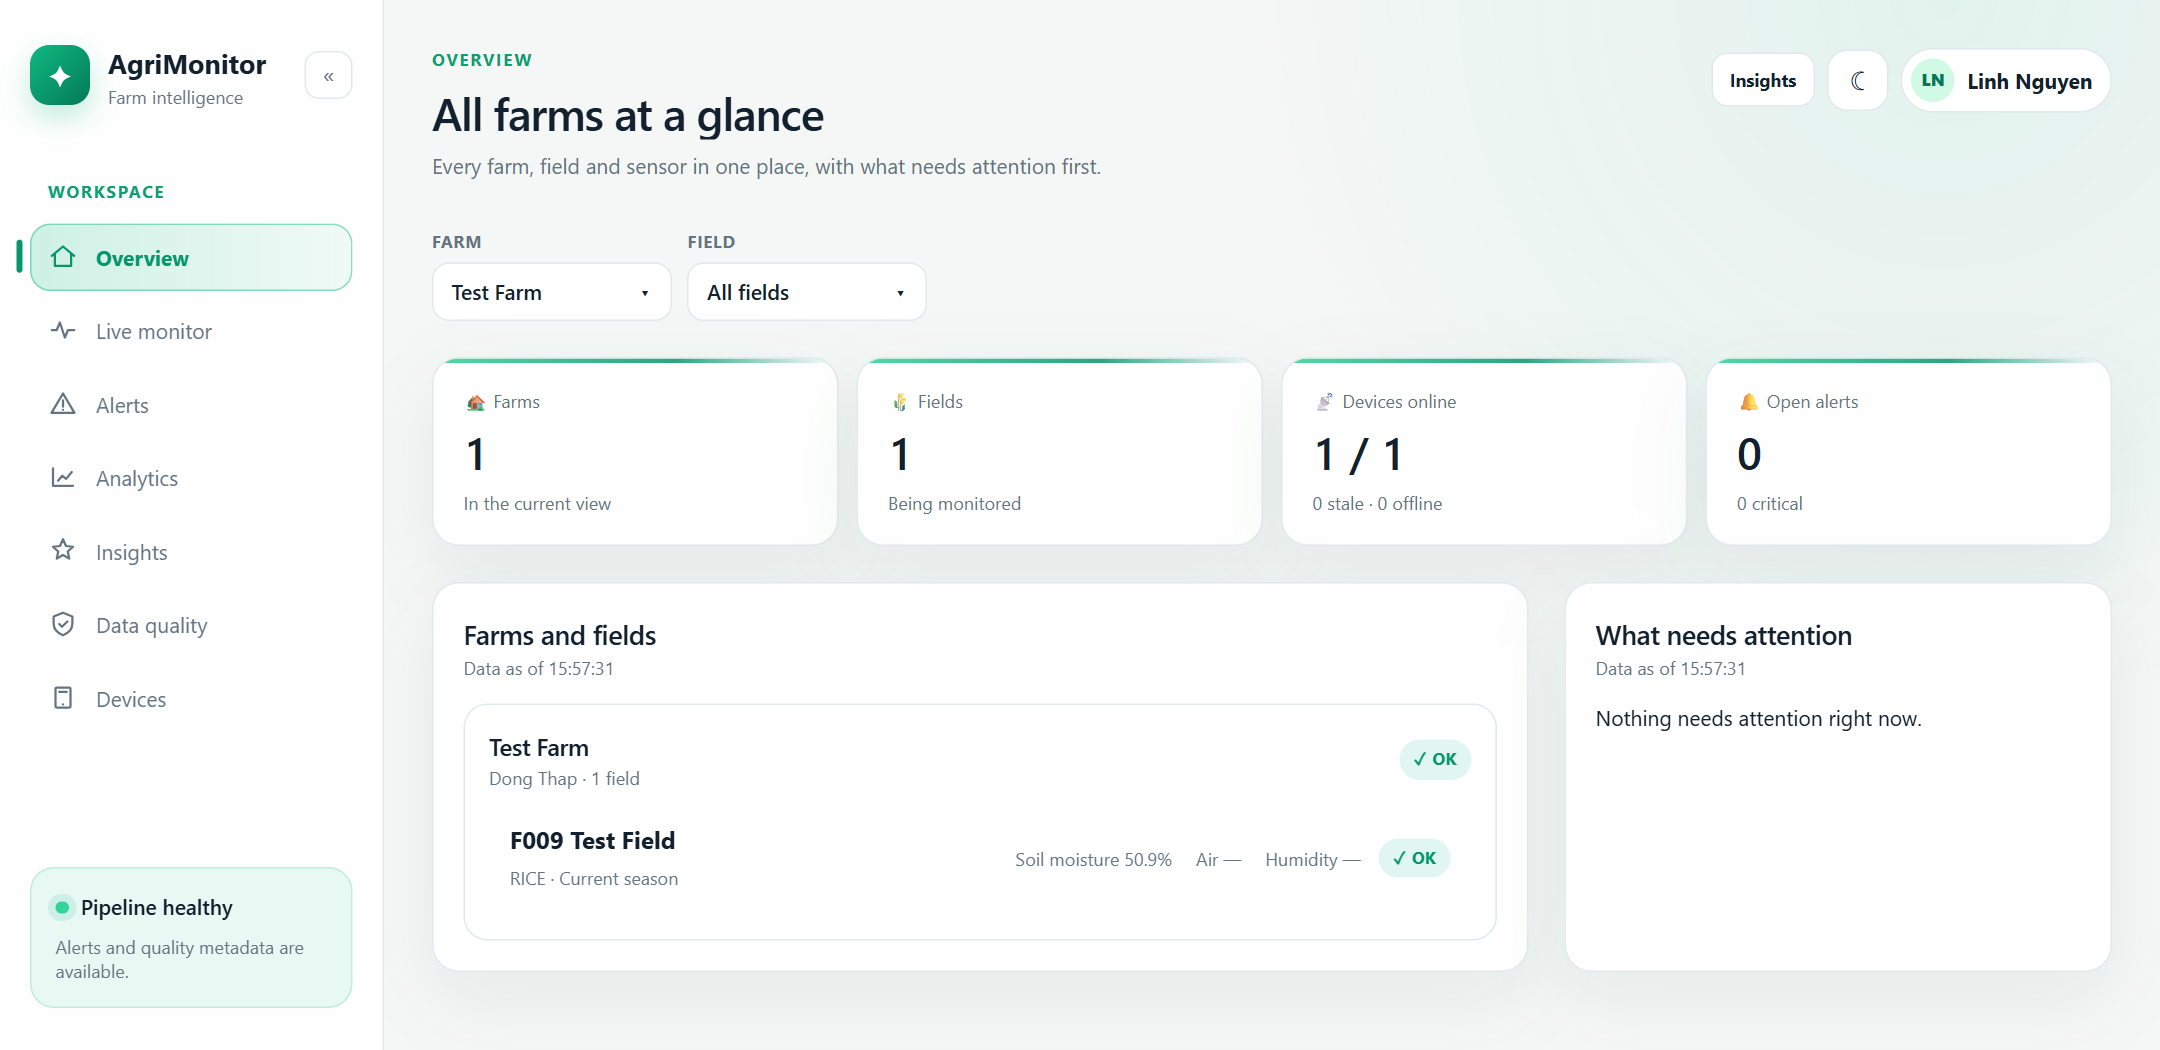
\includegraphics[width=0.85\linewidth]{br01-overview.png}
\caption{Trang Overview sau khi thêm trang trại FM005 vào dữ liệu danh mục}
\label{fig:5-br01-newfield}
\end{figure}

\paragraph{Thiết bị lạ.} Hai số đo của thiết bị F999-S01 được gửi tới service tiếp nhận. Service chấp nhận cả hai (mã 202) vì phía tiếp nhận chỉ kiểm tra hình thức bản ghi. Sau một micro-batch, cả hai bản ghi nằm trong bảng \code{ops.quarantine} với \code{reason = unknown\_device}, cùng \code{event\_id} và nội dung gốc. Truy vấn \code{/fields/F999/latest} trả lỗi 404, tức không có thửa ruộng hay giá trị nào được tạo ra từ chúng.
